\documentclass[a4paper, 11pt]{article}
\usepackage[cpp]{mypackage}
\usepackage{float}
\usepackage{amsmath}
\usepackage{graphicx}
\usepackage{geometry}
\usepackage{listings}
\geometry{scale=0.8}
% \linespread{1.5}
\usepackage{hyperref}
\usepackage{longtable}
\lstset{language=python}

\title{
\normalfont \normalsize
\textsc{School of Data and Computer Science, Sun Yat-sen University} \\ [25pt] %textsc small capital letters
\rule{\textwidth}{0.5pt} \\[0.4cm] % Thin top horizontal rule
\huge  P01 Pacman Game \\ % The assignment title
\rule{\textwidth}{2pt} \\[0.5cm] % Thick bottom horizontal rule
\author{17341015 Hongzheng Chen}
\date{\normalsize\today}
}

\begin{document}
\maketitle
\tableofcontents
\newpage

For the codes, please refer to the attached files.

\section{Question 1: A* search (3 points)}
\texttt{python pacman.py -l bigMaze -z .5 -p SearchAgent -a fn=astar,heuristic=manhattanHeuristic}

\begin{lstlisting}
def aStarSearch(problem, heuristic=nullHeuristic):
    """Search the node that has the lowest combined cost and heuristic first."""
    start = problem.getStartState()
    queue = util.PriorityQueue()
    queue.push((0,start,[]),0)
    visited = []
    while not queue.isEmpty():
        cost, curr, actions = queue.pop()
        if curr in visited:
            continue
        visited.append(curr)
        if problem.isGoalState(curr):
            break
        for succ in problem.getSuccessors(curr):
            priority = cost + succ[2] + heuristic(succ[0],problem)
            queue.push((cost+succ[2],succ[0],actions+[succ[1]]),priority)
    return actions
\end{lstlisting}

\begin{figure}[H]
  \centering
  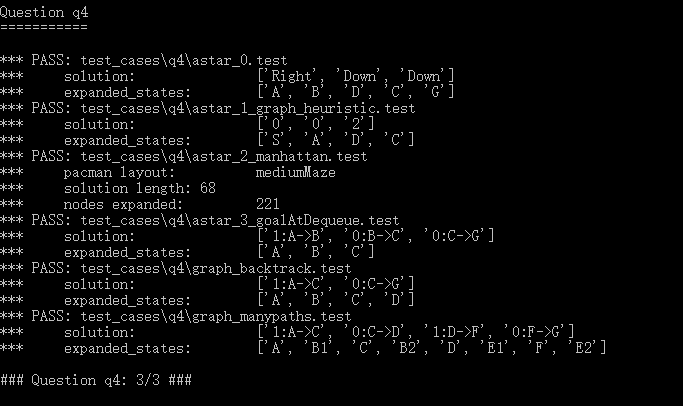
\includegraphics[width=\linewidth]{fig/Q1.png}
\end{figure}

\section{Question 2: Corners Problem: Heuristic (3 points)}
\texttt{python pacman.py -l mediumCorners -p SearchAgent -a fn=aStarSearch,\\prob=CornersProblem,heuristic=cornersHeuristic --frameTime 0}

I represent the state as below
\begin{center}
  pacmanx, pacmany, 0, 0, 0, 0
\end{center}
where the last four numbers indicating whether there is food in the corner.
And the goal state is
\begin{center}
  *, *, 1, 1, 1, 1
\end{center}

Actually, I design lots of heuristic functions which are all listed below.
The best one may be the heuristic that calculates maximum maze distance between current point and unvisited corners (using BFS).
This is obviously admissible and consistent, since every time the pacman reach to a corner, the total distance can be reduced, and the heuristic value of the goal state is 0.
And this is a strategy putting computation on pruning but not searching, where the pruning time may cost a lot.
The result also shows that only 802 nodes are needed to expanded by my heuristics.

\begin{lstlisting}
class CornersProblem(search.SearchProblem):
    """
    This search problem finds paths through all four corners of a layout.

    You must select a suitable state space and successor function
    """

    def __init__(self, startingGameState):
        """
        Stores the walls, pacman's starting position and corners.
        """
        self.walls = startingGameState.getWalls()
        self.startingPosition = startingGameState.getPacmanPosition()
        top, right = self.walls.height-2, self.walls.width-2
        self.corners = ((1,1), (1,top), (right, 1), (right, top))
        for corner in self.corners:
            if not startingGameState.hasFood(*corner):
                print 'Warning: no food in corner ' + str(corner)
        self._expanded = 0 # DO NOT CHANGE; Number of search nodes expanded
        # Please add any code here which you would like to use
        # in initializing the problem
        self.startingGameState = startingGameState
        visited = [0,0,0,0]
        for (i,corner) in enumerate(self.corners):
            if self.startingPosition == corner:
                visited[i] = 1
        self.startState = (self.startingPosition,visited)

    def getStartState(self):
        """
        Returns the start state (in your state space, not the full Pacman state
        space)
        """
        return self.startState

    def isGoalState(self, state):
        """
        Returns whether this search state is a goal state of the problem.
        """
        if state[1] == [1,1,1,1]:
            return True
        return False

    def getSuccessors(self, state):
        """
        Returns successor states, the actions they require, and a cost of 1.

         As noted in search.py:
            For a given state, this should return a list of triples, (successor,
            action, stepCost), where 'successor' is a successor to the current
            state, 'action' is the action required to get there, and 'stepCost'
            is the incremental cost of expanding to that successor
        """

        successors = []
        for action in [Directions.NORTH, Directions.SOUTH, Directions.EAST, Directions.WEST]:
            # Add a successor state to the successor list if the action is legal
            # Here's a code snippet for figuring out whether a new position hits a wall:
            #   x,y = currentPosition
            #   dx, dy = Actions.directionToVector(action)
            #   nextx, nexty = int(x + dx), int(y + dy)
            #   hitsWall = self.walls[nextx][nexty]
            x, y = state[0]
            dx, dy = Actions.directionToVector(action)
            nextx, nexty = int(x + dx), int(y + dy)
            if not self.walls[nextx][nexty]:
                nextCorner = [item for item in state[1]]
                if (nextx,nexty) in self.corners:
                    i = self.corners.index((nextx,nexty))
                    nextCorner[i] = 1
                nextState = ((nextx,nexty),nextCorner)
                successors.append((nextState,action,1))

        self._expanded += 1 # DO NOT CHANGE
        return successors

    def getCostOfActions(self, actions):
        """
        Returns the cost of a particular sequence of actions.  If those actions
        include an illegal move, return 999999.  This is implemented for you.
        """
        if actions == None: return 999999
        x,y= self.startingPosition
        for action in actions:
            dx, dy = Actions.directionToVector(action)
            x, y = int(x + dx), int(y + dy)
            if self.walls[x][y]: return 999999
        return len(actions)


def cornersHeuristic(state, problem):
    """
    A heuristic for the CornersProblem that you defined.

      state:   The current search state
               (a data structure you chose in your search problem)

      problem: The CornersProblem instance for this layout.

    This function should always return a number that is a lower bound on the
    shortest path from the state to a goal of the problem; i.e.  it should be
    admissible (as well as consistent).
    """
    corners = problem.corners # These are the corner coordinates
    walls = problem.walls # These are the walls of the maze, as a Grid (game.py)
    top, right = walls.height-2, walls.width-2

    pos = state[0]
    cornerFlag = state[1]
    ## Heuristic 1 (503)
    # res = 0
    # for i,corner in enumerate(corners):
    #     if not cornerFlag[i]:
    #         res += abs(pos[0] - corner[0]) + abs(pos[1] - corner[1])

    ## Heuristic 2 (1057)
    # remaining_corners = []
    # dis = []
    # num_visited = 0
    # for i,corner in enumerate(corners):
    #     if not cornerFlag[i]:
    #         num_visited += 1
    #         remaining_corners.append(corner)
    #         dis.append(abs(pos[0] - corner[0]) + abs(pos[1] - corner[1]))
    # dis.sort()
    # res = 0 if len(dis) == 0 else dis[0]
    # dis = []
    # for i in range(len(remaining_corners)):
    #     for j in range(i+1,len(remaining_corners)):
    #         a = remaining_corners[i]
    #         b = remaining_corners[j]
    #         dis.append(abs(a[0] - b[0]) + abs(a[1] - b[1]))
    # dis.sort()
    # res += sum(dis[:4-num_visited])

    # # Heuristic 3 (693)
    # # Find a path getting through all the foods
    # remaining_points = []
    # curr_point = pos
    # for i,corner in enumerate(corners):
    #     if not cornerFlag[i]:
    #         remaining_points.append(corner)
    # res = 0
    # while len(remaining_points) > 0:
    #     distance = []
    #     for i,point in enumerate(remaining_points):
    #         distance.append((abs(curr_point[0] - point[0]) + abs(curr_point[1] - point[1]),i))
    #     distance.sort()
    #     res += distance[0][0]
    #     index = distance[0][1]
    #     curr_point = remaining_points[index]
    #     remaining_points = remaining_points[:index] + remaining_points[index+1:] # pop out the point with minimum distance
    # return res

    # Heuristic 4 (1135/802)
    from util import manhattanDistance
    remaining_points = []
    for i,corner in enumerate(corners):
        if not cornerFlag[i]:
            remaining_points.append(corner)
    if len(remaining_points) == 0:
        return 0
    # res = max(map(lambda x:manhattanDistance(pos,x), remaining_points))
    res = max(map(lambda x:mazeDistance(pos,x,problem.startingGameState), remaining_points))
    return res
\end{lstlisting}

We can see that the heuristic is admissible and consistent that it can find the optimal solution the same as what UCS found.
\begin{figure}[H]
  \centering
  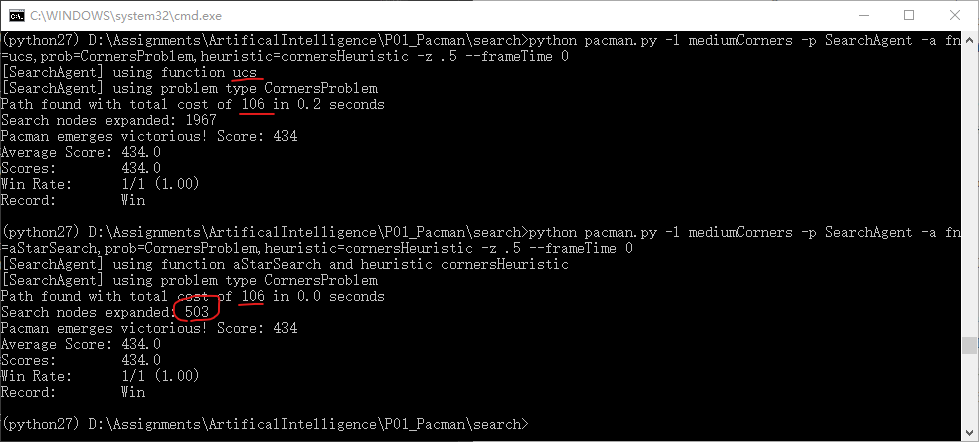
\includegraphics[width=\linewidth]{fig/Q2.png}
\end{figure}

\section{Question 3: Eating All The Dots (4 points)}
\texttt{python pacman.py -l trickySearch -p SearchAgent -a fn=astar,\\prob=FoodSearchProblem,heuristic=foodHeuristic --frameTime 0}.

I reuse the heuristic function in Question 2 that calculates the maximum maze distance from the current position of the pacman to each food.
This is also obviously admissible and consistent, since every time the pacman get to one food, the total distance can be reduced, and the heuristic value of the goal state is 0.
And using this heuristics, only 4111 nodes are expanded.

\begin{lstlisting}
def foodHeuristic(state, problem):

    position, foodGrid = state
    foodLst = foodGrid.asList()
    # print(position) # (10, 3)
    # print(foodLst) # [(1, 1), (1, 4), (1, 5), (2, 1), (3, 1), (4, 1), (4, 4), (5, 1), (7, 4), (10, 4), (13, 4), (13, 5), (14, 5)]

    ## Heuristic 1 (5403)
    # sumup = 0
    # for food in foodLst:
    #     sumup += abs(position[0] - food[0]) + abs(position[1] - food[1])
    # return sumup

    # # Heuristic 2 (6101)
    # remaining_points = [food for food in foodLst]
    # curr_point = position
    # res = 0
    # # Find a path getting through all the foods
    # while len(remaining_points) > 0:
    #     distance = []
    #     for i,point in enumerate(remaining_points):
    #         distance.append((abs(curr_point[0] - point[0]) + abs(curr_point[1] - point[1]),i))
    #     distance.sort()
    #     res += distance[0][0]
    #     index = distance[0][1]
    #     curr_point = remaining_points[index]
    #     remaining_points = remaining_points[:index] + remaining_points[index+1:] # pop out the point with minimum distance
    # return res

    # Heuristic 3 (9445/4111)
    from util import manhattanDistance
    if len(foodLst) == 0:
        return 0
    # res = max(map(lambda x:manhattanDistance(position,x), foodLst))
    res = max(map(lambda x:mazeDistance(position,x,problem.startingGameState), foodLst))
    return res
\end{lstlisting}

We can see that the heuristic is admissible and consistent that it can find the optimal solution the same as what UCS found.
\begin{figure}[H]
  \centering
  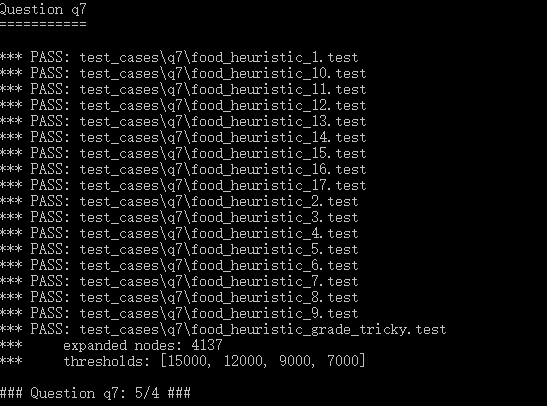
\includegraphics[width=\linewidth]{fig/Q3.png}
\end{figure}

\section{Question 4: Minimax (5 points)}
\texttt{python autograder.py -q q2 --no-graphics}
\begin{lstlisting}
  class MinimaxAgent(MultiAgentSearchAgent):

    def DFMinimax(self, depth, gameState, currAgent):
        actions = gameState.getLegalActions(currAgent)
        if depth > self.depth or len(actions) == 0:
            return (self.evaluationFunction(gameState),Directions.STOP)
        if currAgent == 0: # MAX node
            maxVal = []
            for action in actions:
                state = gameState.generateSuccessor(currAgent,action)
                maxVal.append((self.DFMinimax(depth,state,1)[0],action))
            return max(maxVal)
        else: # MIN node
            minVal = []
            for action in actions:
                state = gameState.generateSuccessor(currAgent,action)
                if currAgent == gameState.getNumAgents() - 1:
                    minVal.append((self.DFMinimax(depth+1,state,0)[0],action))
                else: # one by one action
                    minVal.append((self.DFMinimax(depth,state,currAgent+1)[0],action))
            return min(minVal)

    def getAction(self, gameState):
        _, action = self.DFMinimax(1,gameState,0)
        return action
\end{lstlisting}

The figure below shows my agent passes all the tests.
\begin{figure}[H]
  \centering
  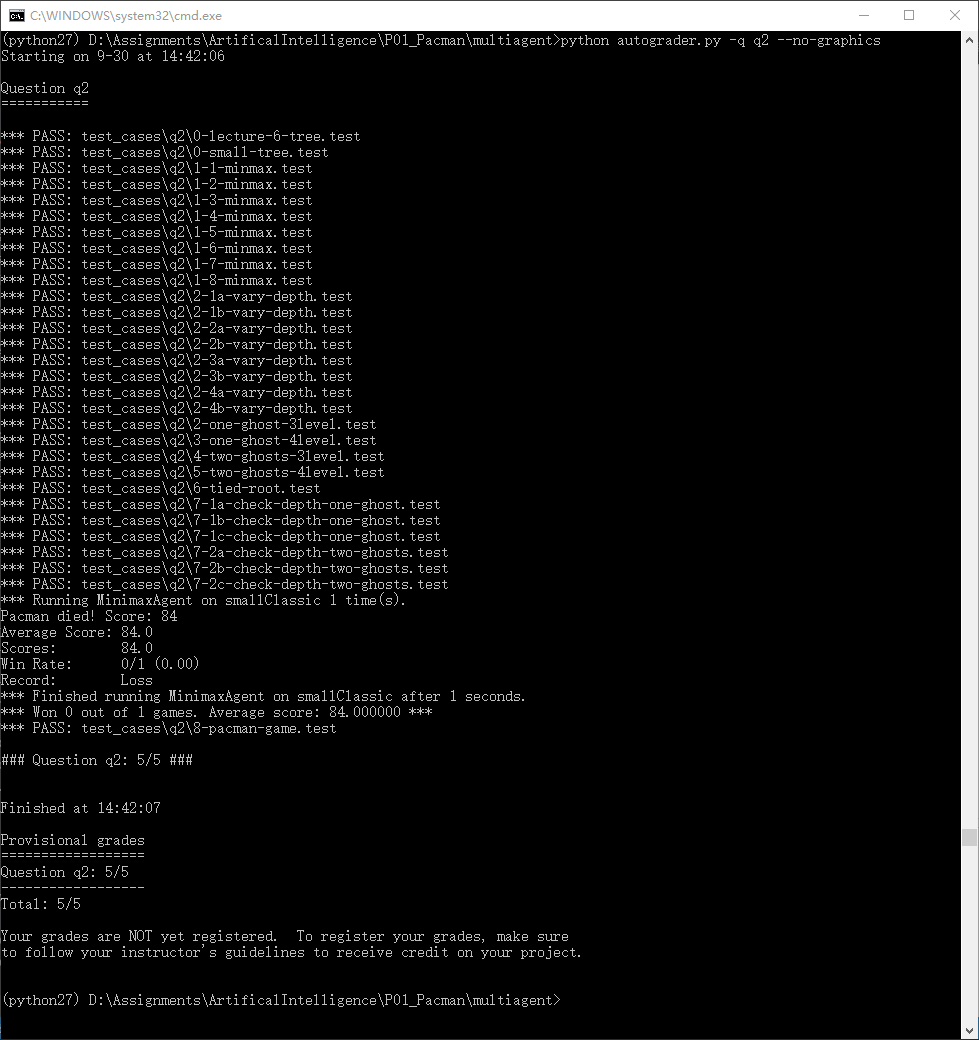
\includegraphics[width=\linewidth]{fig/Q4.png}
\end{figure}

\section{Question 5: $\alpha-\beta$ Pruning (5 points)}
\texttt{python autograder.py -q q3 --no-graphics}
\begin{lstlisting}
  class AlphaBetaAgent(MultiAgentSearchAgent):

    def DFMinimax(self, depth, gameState, currAgent, alpha, beta):
        actions = gameState.getLegalActions(currAgent)
        if depth > self.depth or len(actions) == 0:
            return (self.evaluationFunction(gameState),Directions.STOP)
        if currAgent == 0: # MAX node
            val = (-0x3f3f3f3f,Directions.STOP)
            for action in actions:
                state = gameState.generateSuccessor(currAgent,action)
                val = max(val,(self.DFMinimax(depth,state,1,alpha,beta)[0],action))
                if val[0] > beta:
                    return val
                alpha = max(alpha,val[0])
            return val
        else: # MIN node
            val = (0x3f3f3f3f,Directions.STOP)
            for action in actions:
                state = gameState.generateSuccessor(currAgent,action)
                if currAgent == gameState.getNumAgents() - 1:
                    val = min(val,(self.DFMinimax(depth+1,state,0,alpha,beta)[0],action))
                else: # one by one action
                    val = min(val,(self.DFMinimax(depth,state,currAgent+1,alpha,beta)[0],action))
                if val[0] < alpha:
                    return val
                beta = min(beta,val[0])
            return val

    def getAction(self, gameState):
        _, action = self.DFMinimax(1,gameState,0,-0x3f3f3f3f,0x3f3f3f3f)
        return action
\end{lstlisting}

The figure below shows my agent passes all the tests.
\begin{figure}[H]
  \centering
  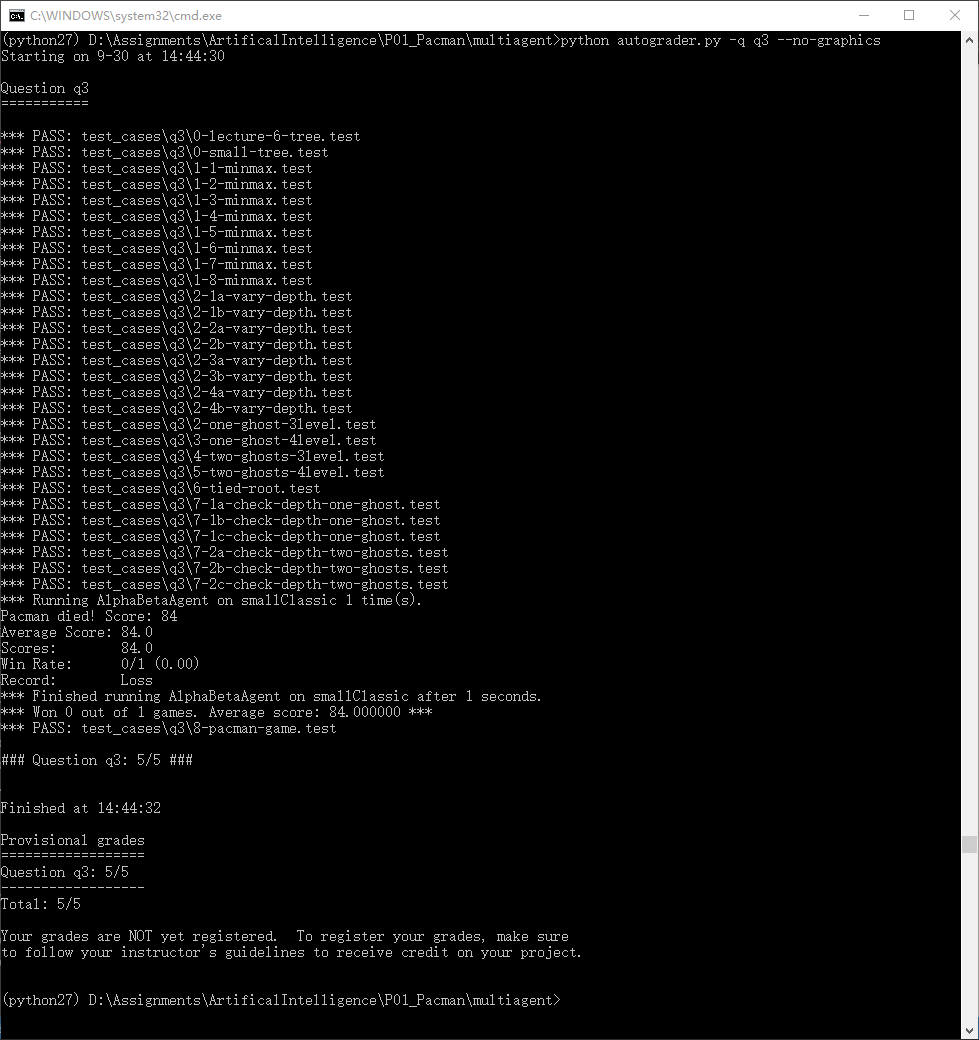
\includegraphics[width=\linewidth]{fig/Q5.png}
\end{figure}


\end{document}